%%%%%%%%%%%%%%%%%%%%%%%%%%%%%%%%%%%%%%%%%%%%%%%%%%%%%%%%%%%%%%%%%%%%%%%%%%%

\documentclass{standalone}

\usepackage{amsmath}
\usepackage{mathptmx}
\usepackage{pgfplots}
\usetikzlibrary{external}
\tikzexternalize{sunshine-vary-c-ignore-highest}
\pgfplotsset{compat=1.16}

%% IEEE uses Times Roman font, so we'll default to Times.
%% These three commands make up the entire times.sty package.
\renewcommand{\rmdefault}{ptm}
\renewcommand{\ttdefault}{pcr}
\normalfont\selectfont

\begin{document}

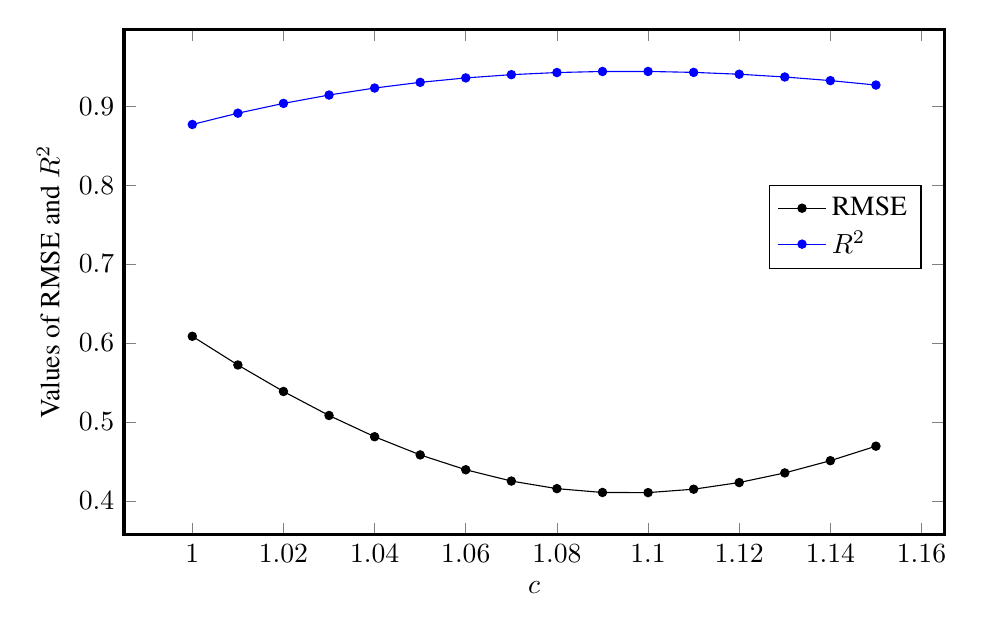
\begin{tikzpicture}
\tikzset{%%
  every mark/.append style={scale=1.0},%%
  scale=1.0%%
}
\pgfplotsset{%%
  every axis/.append style={font=\normalsize}%%
}
%%
\begin{axis}[%%
  axis line style=very thick,%%
  dotStyle/.style={mark size=1.5,mark color=black,mark=*},%%
  enlargelimits=true,%%
  height=8cm,%%
  legend cell align=left,%%
  legend style={at={(axis cs:1.16,0.8)},anchor=north east},%%
  width=12cm,%%
  %% x axis
  xlabel={\normalsize $c$},%%
  %% y axis
  ylabel={\normalsize Values of RMSE and $R^2$}%%
]
%%
%%
%% The change in the values of the RMSE.
\addplot[dotStyle,black] coordinates {
  (1.00, 0.608533)
  (1.01, 0.572170)
  (1.02, 0.538615)
  (1.03, 0.508211)
  (1.04, 0.481317)
  (1.05, 0.458297)
  (1.06, 0.439491)
  (1.07, 0.425185)
  (1.08, 0.415572)
  (1.09, 0.410721)
  (1.10, 0.410555)
  (1.11, 0.414860)
  (1.12, 0.423307)
  (1.13, 0.435493)
  (1.14, 0.450986)
  (1.15, 0.469360)
};
\addlegendentry{RMSE}
%%
%%
%% The change in the values of R^2.
\addplot[dotStyle,blue] coordinates {
  (1.00, 0.876756)
  (1.01, 0.891045)
  (1.02, 0.903450)
  (1.03, 0.914043)
  (1.04, 0.922899)
  (1.05, 0.930098)
  (1.06, 0.935717)
  (1.07, 0.939834)
  (1.08, 0.942524)
  (1.09, 0.943858)
  (1.10, 0.943903)
  (1.11, 0.942721)
  (1.12, 0.940364)
  (1.13, 0.936881)
  (1.14, 0.932311)
  (1.15, 0.926682)
};
\addlegendentry{$R^2$}
\end{axis}
\end{tikzpicture}

\end{document}
